\documentclass{article}
\usepackage{graphicx}
\usepackage{amsmath}
\usepackage{geometry}
\geometry{a4paper, margin=1in}

\title{Aerodynamic Optimization Report}
\author{LLM Analysis}
\date{2025-05-25}

\begin{document}
\maketitle

\section{Executive Summary}
This report details the aerodynamic optimization performed to minimize drag on a wing while maintaining a lift coefficient of 2.0. The wing area was constrained to 100 $m^2$ and the span to 10 m. The optimization process considered taper, twist, and sweep as design variables. The optimization converged successfully, achieving a drag coefficient of 0.01097. The lift distribution is close to elliptical, indicating an efficient design. However, a higher-fidelity analysis is recommended to validate these results, along with exploration of constraint boundaries.

\section{Problem Formulation}
The optimization problem was defined as follows:
\begin{itemize}
    \item Objective Function: Minimize Drag ($C_D$)
    \item Trim Condition: Lift Coefficient ($C_L$) = 2.0
    \item Geometric Constraints: Wing Area (S) = 100 $m^2$, Span (b) = 10 m
    \item Design Variables: Taper Ratio, Twist Distribution, Sweep Angle
    \item Baseline Wing Mesh: Rectangular
    \item Optimization Algorithm: SLSQP
\end{itemize}

\section{Optimization Results}
The optimization process converged in 11 iterations using the SLSQP optimizer. Key optimized parameters include:
\begin{itemize}
    \item Taper Ratio: 0.2 (lower bound)
    \item Sweep Angle: 28.5 degrees (upper bound)
    \item Twist Distribution: Values between 1.46 and 2.47 degrees
\end{itemize}

The resulting drag coefficient ($C_D$) was 0.01097. The elliptical lift distribution plot indicates an efficient design, although not perfectly elliptical due to geometric constraints.  The optimized wing design is visualized in Figure \ref{fig:Optimized_Wing}.

\begin{figure}[h!]
    \centering
    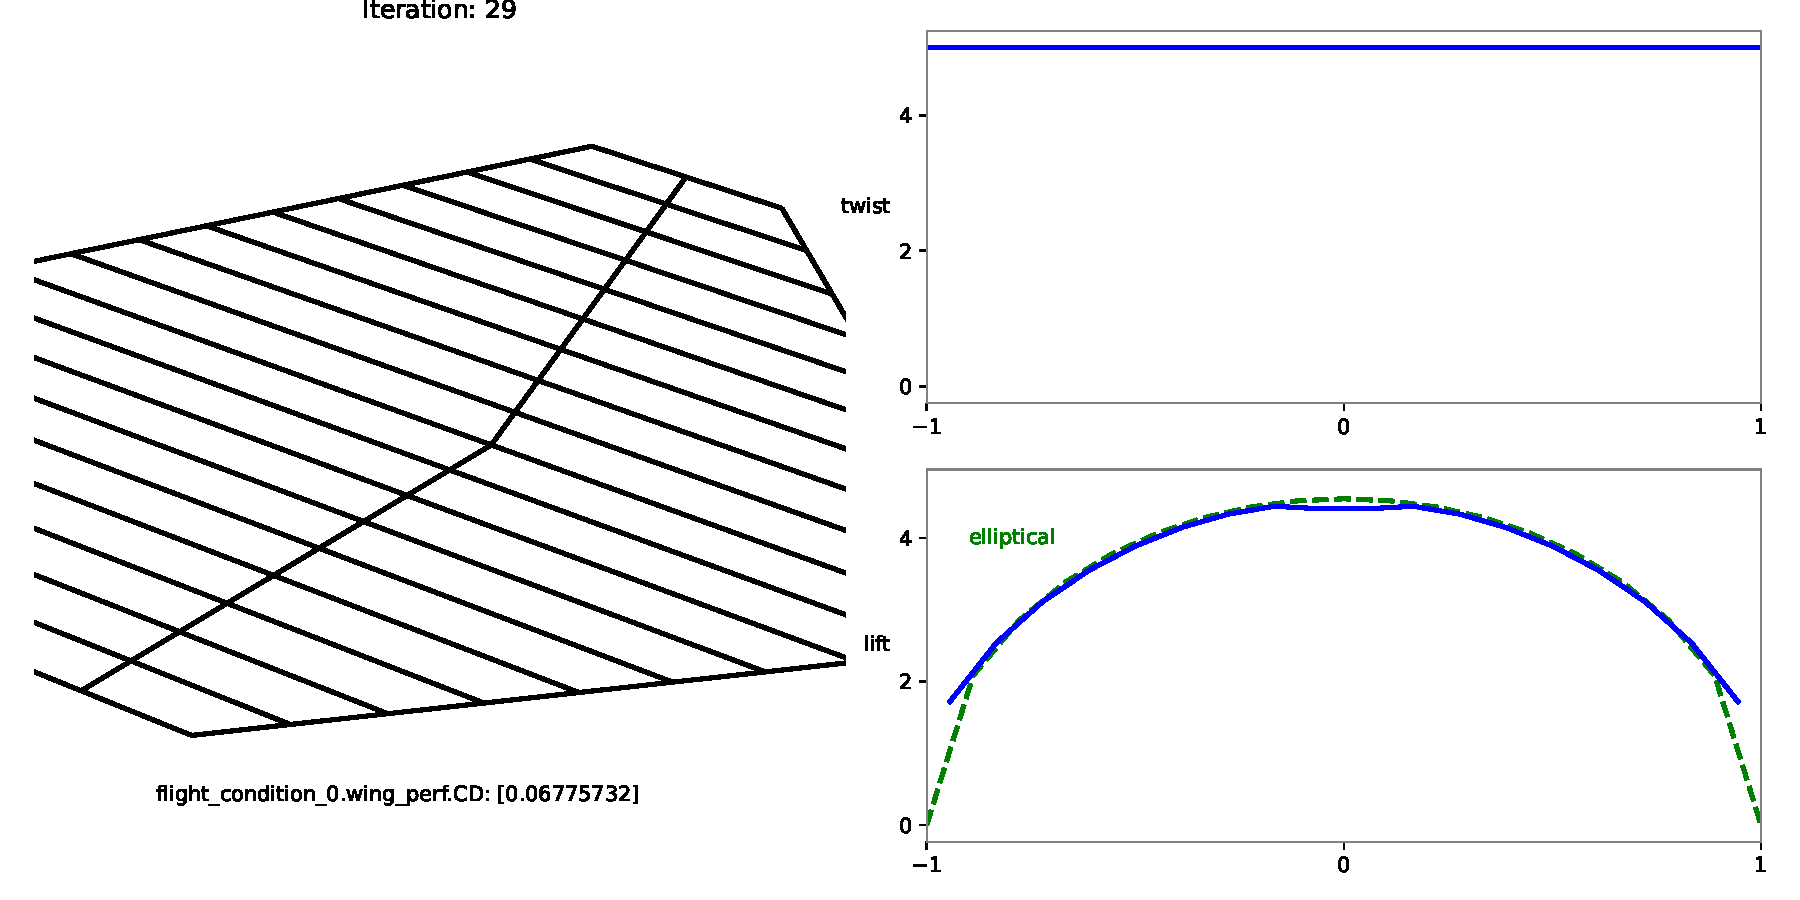
\includegraphics[width=0.75\textwidth]{./Figures/Optimized_Wing.pdf}
    \caption{Optimized Wing Visualization}
    \label{fig:Optimized_Wing}
\end{figure}

\section{Analysis and Recommendations}
Based on the optimization results, the following recommendations are made:
\begin{enumerate}
    \item \textbf{Higher Fidelity Analysis:} Conduct a higher-fidelity CFD analysis to validate the drag reduction and lift characteristics, as the current results are based on the Vortex Lattice Method (VLM).
    \item \textbf{Explore Taper Ratio Lower Bound:} Re-run the optimization with a lower or no lower bound on the taper ratio to potentially further reduce drag, as the current optimization hit the lower bound.
    \item \textbf{Explore Sweep Upper Bound:} Relax the upper bound on the sweep angle to assess its impact on drag reduction, since the optimization reached the upper bound.
    \item \textbf{Airfoil Optimization:} Incorporate airfoil shape optimization to further enhance aerodynamic performance. OpenAeroStruct does not have this feature, consider adding it.
    \item \textbf{Structural Analysis:} Perform a structural analysis to ensure the optimized wing can withstand the aerodynamic loads. OpenAeroStruct has built-in structural optimization capabilities which may be added.
    \item \textbf{Manufacturability Assessment:} Evaluate the manufacturability of the optimized wing, considering the complexity of high twist and highly tapered designs.
\end{enumerate}

\section{Optimization Performance}
The SLSQP optimizer demonstrated fast convergence, completing in 11 iterations with negligible wall-clock run time. This suggests SLSQP is a suitable optimizer for this problem. However, for more complex scenarios with additional constraints or objectives, alternative optimizers such as SNOPT or IPOPT may be considered.

\section{Limitations}
It is crucial to acknowledge the limitations of the VLM, particularly in capturing stall and viscous effects. The absolute drag values should be interpreted with caution, as VLM may underestimate total drag and stall effects. The elliptical lift distribution is a theoretical ideal, and practical geometric constraints may prevent achieving it perfectly.

\end{document}